\documentclass[12pt]{article}
\usepackage{graphicx}
\usepackage{caption}
\usepackage{amsmath}
\usepackage{bibtopic}
\usepackage{hyperref}


\begin{document}

\setlength\parindent{0pt}
\title{Raw Audio Music Generation Using Deep Neural Networks}
\author{Fabian Stahl}


\maketitle

\tableofcontents

\newpage
\section*{Abbreviations}
\begin{center}
\begin{tabular}{l l}
\textbf{CNN} & Convolutional neural network \\
\textbf{DCGAN} & Deep Convolutional Generative Adverserial Networks\\
\textbf{GAN} & Generative adversarial network \\
\textbf{GRU} & Gated Recurrent Unit \\
\textbf{KLD}  & Kullback–Leibler divergence\\
\textbf{LSTM} & Long short-term memory \\
\textbf{MIDI} & Musical Instrument Digital Interface \\
\textbf{MLP} & Multilayer Perceptrons \\
\textbf{ReLU} & Rectified Linear Unit \\
\textbf{RNN} & Recurrent neural network \\
\textbf{VAE} & Variational autoencoder \\
\textbf{VRNN} & Variational Recurrent neural network \\
\end{tabular}
\end{center}
\newpage


\begin{abstract}
Music can be found in almost every movie, video game or public location.
Its targeted use can change people's mood, encourage buying decisions or add context to accompanying content.
However, composing, recording and mixing music is a creative process, that takes a lot of time and skill to master.
This poses the question, if pleasing music can be generated autonomously.

Deep neural networks have been known to solve a wide range problems.
During this semester's project I will compare different network architectures to generate sample based music, show how they can be trained and rate results.
\end{abstract}

\section{Related Work}
% midi
In the field of audio generation there is a wide variety of approaches.
Most of them work with symbolic music representations, such as Ascii-text, musical scores or spectrogram data.
Especially the MIDI format is commonly used, a binary format specifying musical notes.
This makes the format very slim and easy to work with.
MIDI-based approaches include e.g. GANs with convolutions layers ~\cite{yang2017midinet, mogren2016c, mogren2016c}, VAEs paired with LSTMs~\cite{roberts2018hierarchical, tikhonov2017music, hennig2017classifying} and RNNs with restricted Boltzmann machines \cite{boulanger2012modeling}.
However, musical nuances like tonal colors, scratch and breath noises or intonations are necessary to make most music genres more interesting.
Having MIDI output only, the musical interpretation, (the raw audio sent to the sound port), is up to an external MIDI synthesizer.

There are commercial music streaming services that claim to provide generated music that fits the customer's mood.
The most prominent of them being brain.fm~\cite{brain.fm} and \cite{mubert}.
However, the brain.fm algorithm only learns certain tasks, such as arranging motifs over long timescales, while melodies, instrument choices and chord progressions are pre-composed by humans.
Mubert also uses handcrafted single instrument MIDI loops, but generates some MIDI layers using decision trees, random forests and musical analysis.
Their music is limited to electronic genres only, which narrows musical variety.
While these application developers like to emphasize the machine learning aspect, their algorithms are not fully autonomous.
The two biggest reasons for that could be the high complexity of generating music sample by sample, especially with real time constraints, as well as the ineptitude of the synthesized music for commercial use.




\section{SampleRNN}
Recurrent Neural Networks (RNNs) are used to process sequences of data.
Output data is not only based upon input data, but also on a hidden state vector, that encodes previous input.
RNNs consist of arrays of small memory units.
While the original \emph{vanilla cells} were prone to the vanishing gradient problem, more advanced structures like LSTMs and GRUs could learn to keep important information and forget redundant or irrelevant previous input.

In audio data correlation can exist between neighbouring samples as well as between samples that are more than thousand frames apart.
Mehri et al. states that common RNNs don't scale very good with a very high temporal resolution and proposes to use multiple hierarchical stacked RNNs with different temporal resolutions to capture all audio features~\cite{mehri2016samplernn} (see \ref{fig:samplernn-arch} for an example model).
This model is called \emph{SampleRNN}.
Originally tested only for piano music, \cite{zukowski2018generating} and \cite{carr2018generating} showed, that SampleRNN is especially good to generate loud music genres, like Metal and Dark Ambient.
This makes the \textbf{SampleRNN} a promising candidate for music generation.

The implementation used in this work was built on top of a project called \emph{Deepsound-project}~\cite{samplernn-git}.
However, in a few cases this version differs from the original proposal.
Main differences include
\begin{itemize}
 \item works with an arbitrary number of frame-level tiers
 \item 1D convolutions instead of fully-connected layers
 \item upsampling layers prior to RNN cells
\end{itemize}



\subsection{Architecture}
The (Deepsound-project) SampleRNN consists of multiple hierarchicaly stacked \emph{Frame-Level Modules} and a single \emph{Sample-Level Moudle}.
Each Frame-Level Module is an RNN that generates a conditioning vector for the next lower tier based on a state vector that summerizes previous input.
The same audio data is passed to all Modules, but while the number of chunks increases with the lower tiers, the chunks itself become smaller.
At the bottom of the model is a single \emph{Sample-Level Module}.
It puts the combined conditioning vector from above into consideration as well as the raw audio samples to generate probability distribution for each chunk.

At generation time the Sample Level Module is run repeatedly, where each sample is fed back into the model.
Conditioning vectors from the Frame Level Modules are refreshed using a lower clock rate if enough samples are generated to have a new non-overlapping input chunk for the RNNs.


\subsection{Training}
To allow an efficient training of the model, truncated backpropagation through time is used.
Since it is computational very expensive to propagate gradients back after a full song, training on shorter subsequences of 8 seconds is much more feasible. % To-Do - how??
The initial state vectors of all GRUs was learned.

Figure \ref{fig:samplernn-arch} shows a training cicle of a model with the following parameters:
\begin{center}
\begin{tabular}{ r | l | l }
variable name & value & description \\
\hline
frame sizes & 16, 4 & numbers of Frame-Level chunks per upper tier chunk\\
sequence length & 1024 & how many samples to include in each training step\\
quatization levels & 256 & number of bins in quantization of audio samples\\
num rnns & 3 & number of stacked GRUs per Frame-Level \\% To-DO! Change in image
dim & 1024 & dimension of the state vectors $h$, neurons in Sample-Level \\
learning rate & 0.001 & \\
batch size & 128 & \\
sample rate & 16000 & \\
\end{tabular}
\end{center}

First the top Frame Level Module chunks the input data into 16 chunks, each having 64 samples. 
Using a 1D convolution each 64 sample chunk is expanded to a 1024 sample chunk (1).
These chunks are fed into three stacked GRUs, that predict the follow up sequences based on a state vector $h$ (2).
To be able to pass the condition vectors to the next lower tier with a faster clock rate, a transpose 1D convolution helps to upsample 16 to 64 chunks (3).
The middle tier repeats step 1, but uses a smaller clock rate (64 chunks, each with 16 samples) and adds the expanded result to the conditioning vector from above (4).
The signal than passes the midle tier GRU and upsampling layers.
The Sample-Level module first quantizes the whole input sequence to 256 levels and maps each bin to a real-values vector embedding (5).
This signal is passed through a 1D convolution to match the conditioning signal from the middle tier (6).
The combined signal passes a MLP (expressed with 1D convolutions) as well as a Softmax layer to calculte probability distributions (7).
According to \cite{mehri2016samplernn} a discrete output distribution using a q-way Softmax yields better results than a dense distribution using for example Gaussian Mixture Models.
Finally the output signal is compared to the ground truth data and the negative log likelihood (NLL) is calculated.
Based on this score the Adam optimizer adjusts the models parameters (8). 


SampleRNN experiments were stopped after $???$ steps since no more progress was achieved.
On a NVIDIA RTX2080 GPU, this took about $???$ and almost the full 8Gb RAM.

\begin{figure}[ht!]
    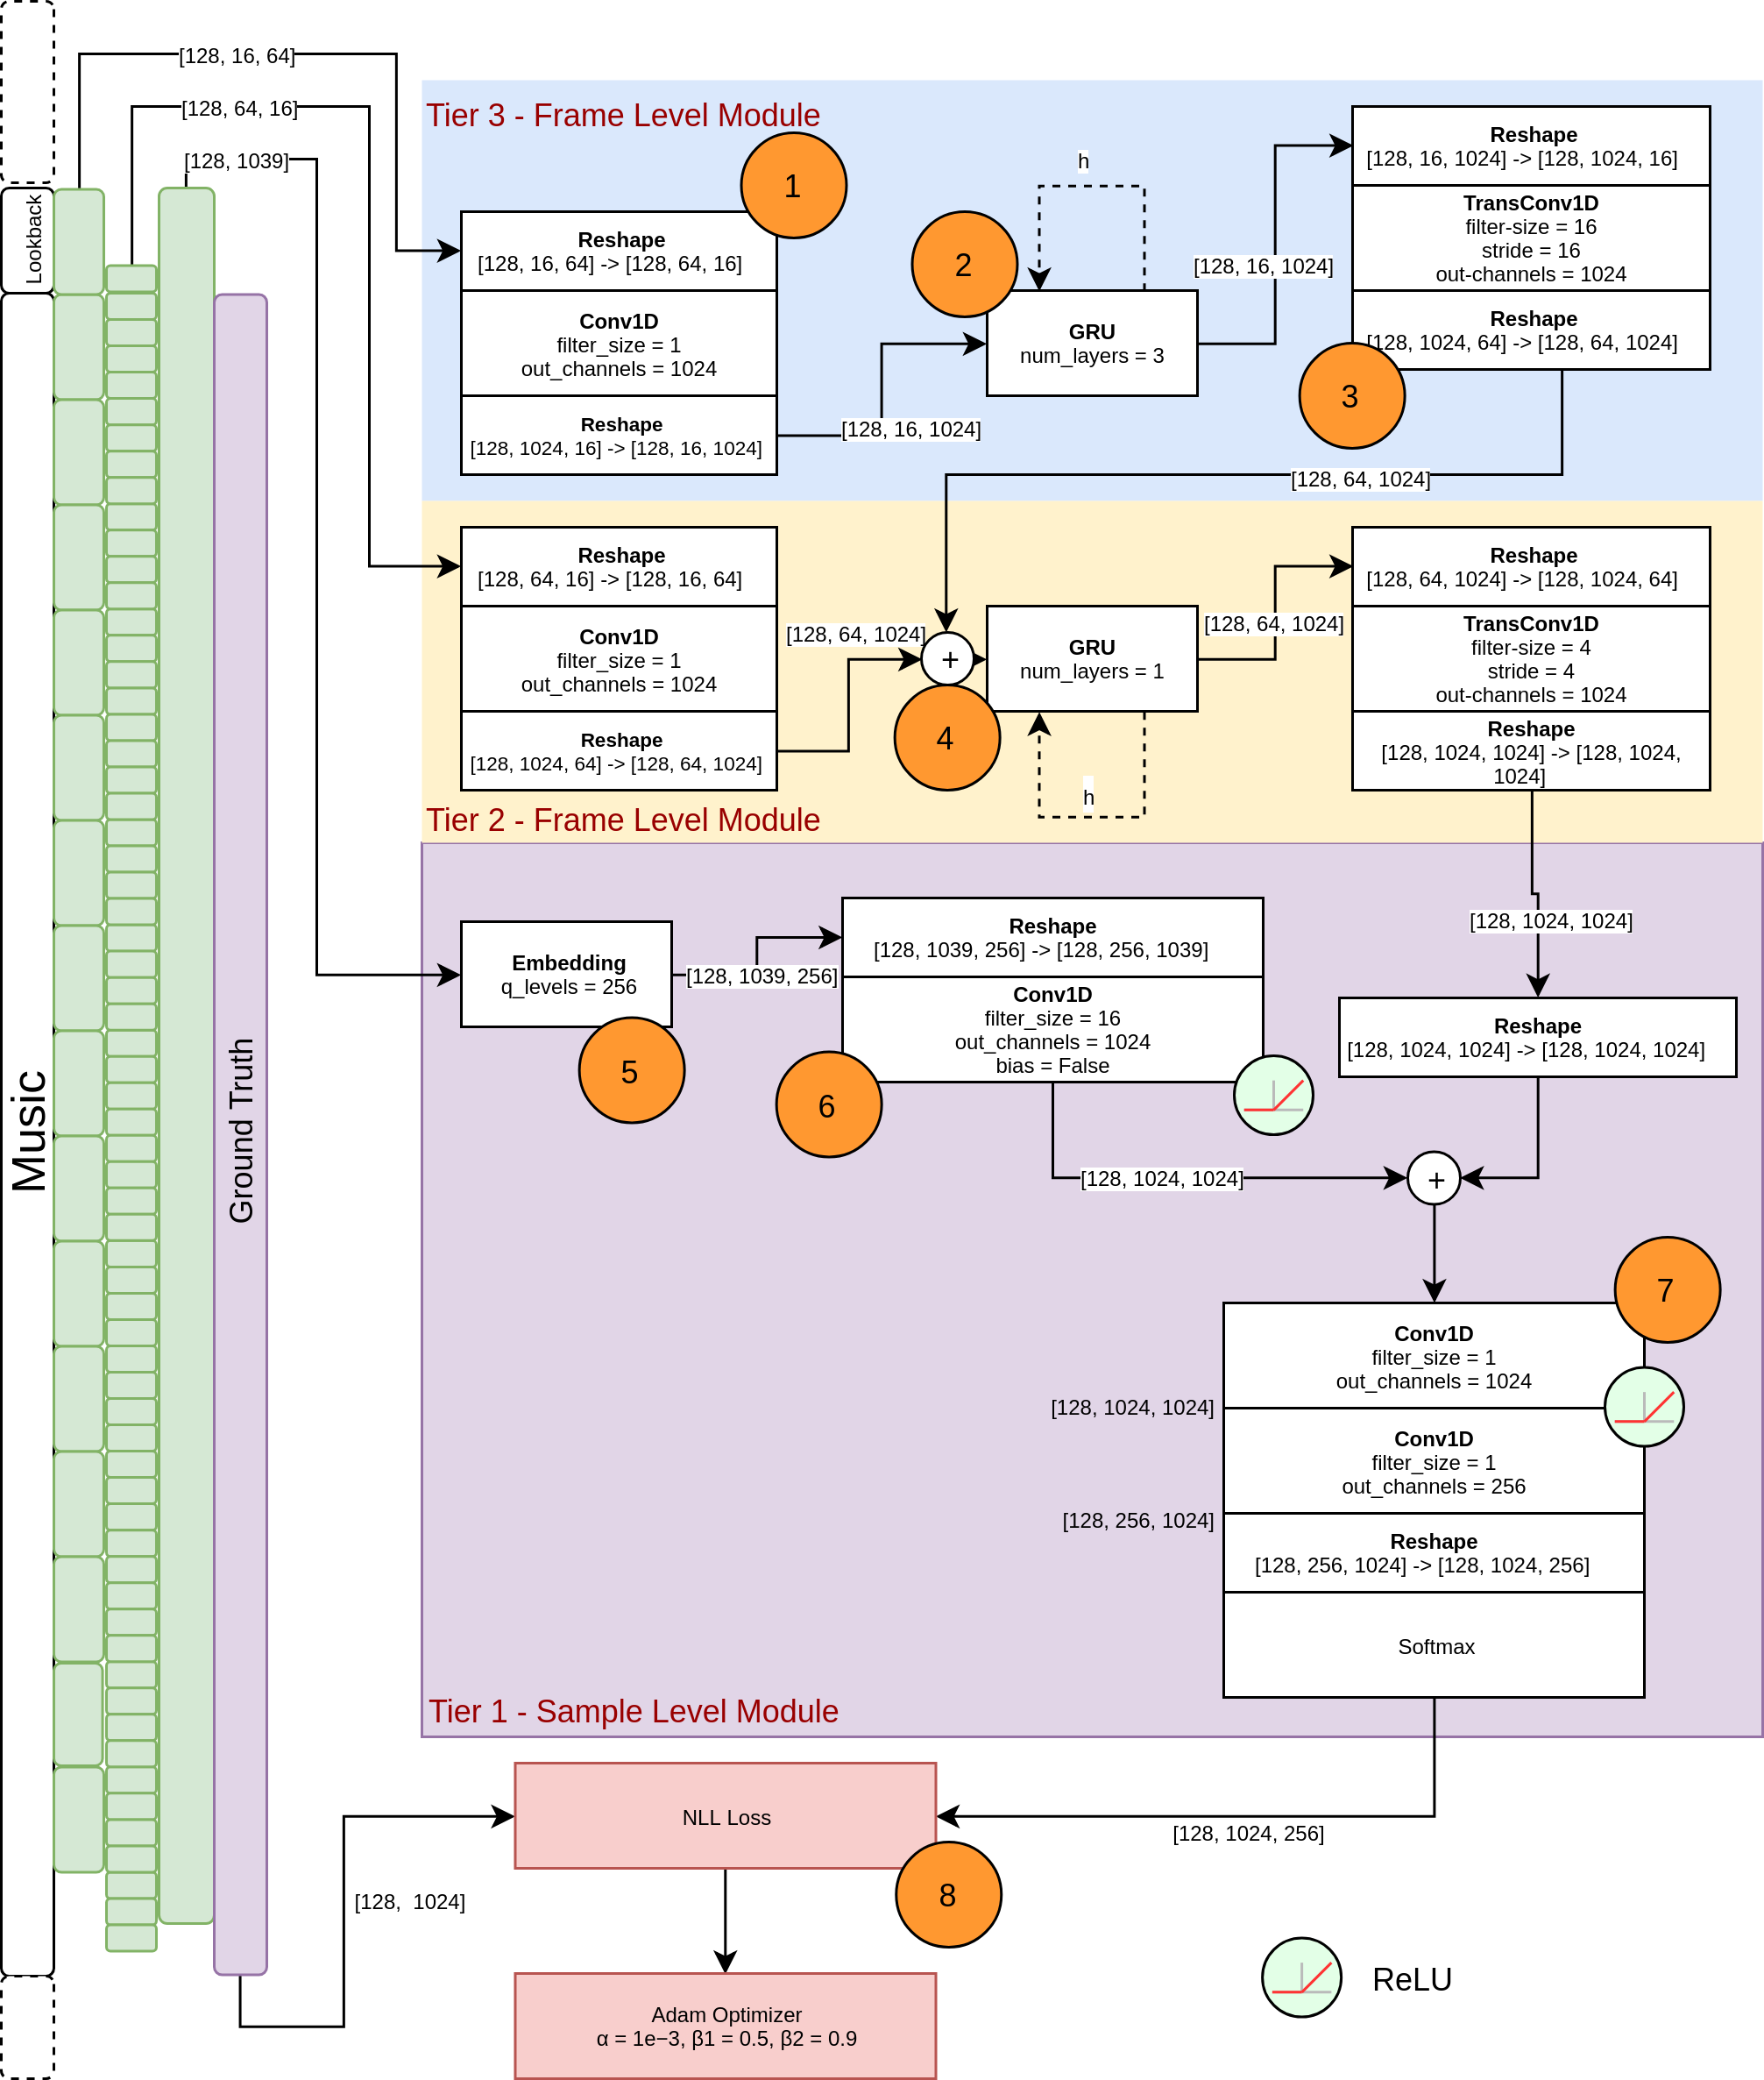
\includegraphics[width=\textwidth]{img/samplernn-arch.png}
    \caption{No caption} % To-DO
    \label{fig:samplernn-arch}
\end{figure}



\section{VRNN}

% Idee (Markov, variational autoencoder erklären)
\subsection{Idea}
Another approach to generate sound data is the Variational Recurrent Neural Network (VRNN), proposed 2016 by Chung et al.~\cite{chung2015recurrent}.
The architecture was trained on the tasks of handwriting and sound generation.
However, experiments for the ladder only included training with speech datasets and non-linguistic human-made sounds like coughing and screaming.
This poses the question if the VRNN can be used to generate music as well.

Chung et al. states that there is an issue in the way that RNNs model output variety, since the only source of true randomness is drawing values from an output probability density.
Data that is both highly variable and highly structered can be hard to model this way.
On the one hand small input variations should lead to potentially very large variations in the hidden state vector $h_t$, on the other hand, different high level structures need to be mapped to distinct state vectors as well.
This forces the network to compromise between the encoding of low-level and high-level features.
The main idea of the VRNN is to extend a recurrent neural network with latent random variables, therefore improving the representational power of the model.
Such high-level variables are commonly used in VAEs to model multimodal conditional distributions, approximating real world data variety~\cite{kingma2013auto}.
% <Satz zu VAEs>
Chung et al. proposes to extend the VEA model by inducing temporal dependencies using the hidden state vector of a RNN across neighboring timesteps.



 
% Architektur erklären (Diagramme, Fehlerfunktionen, Trainingsdiagramme)



\subsection{Training}

\begin{figure}
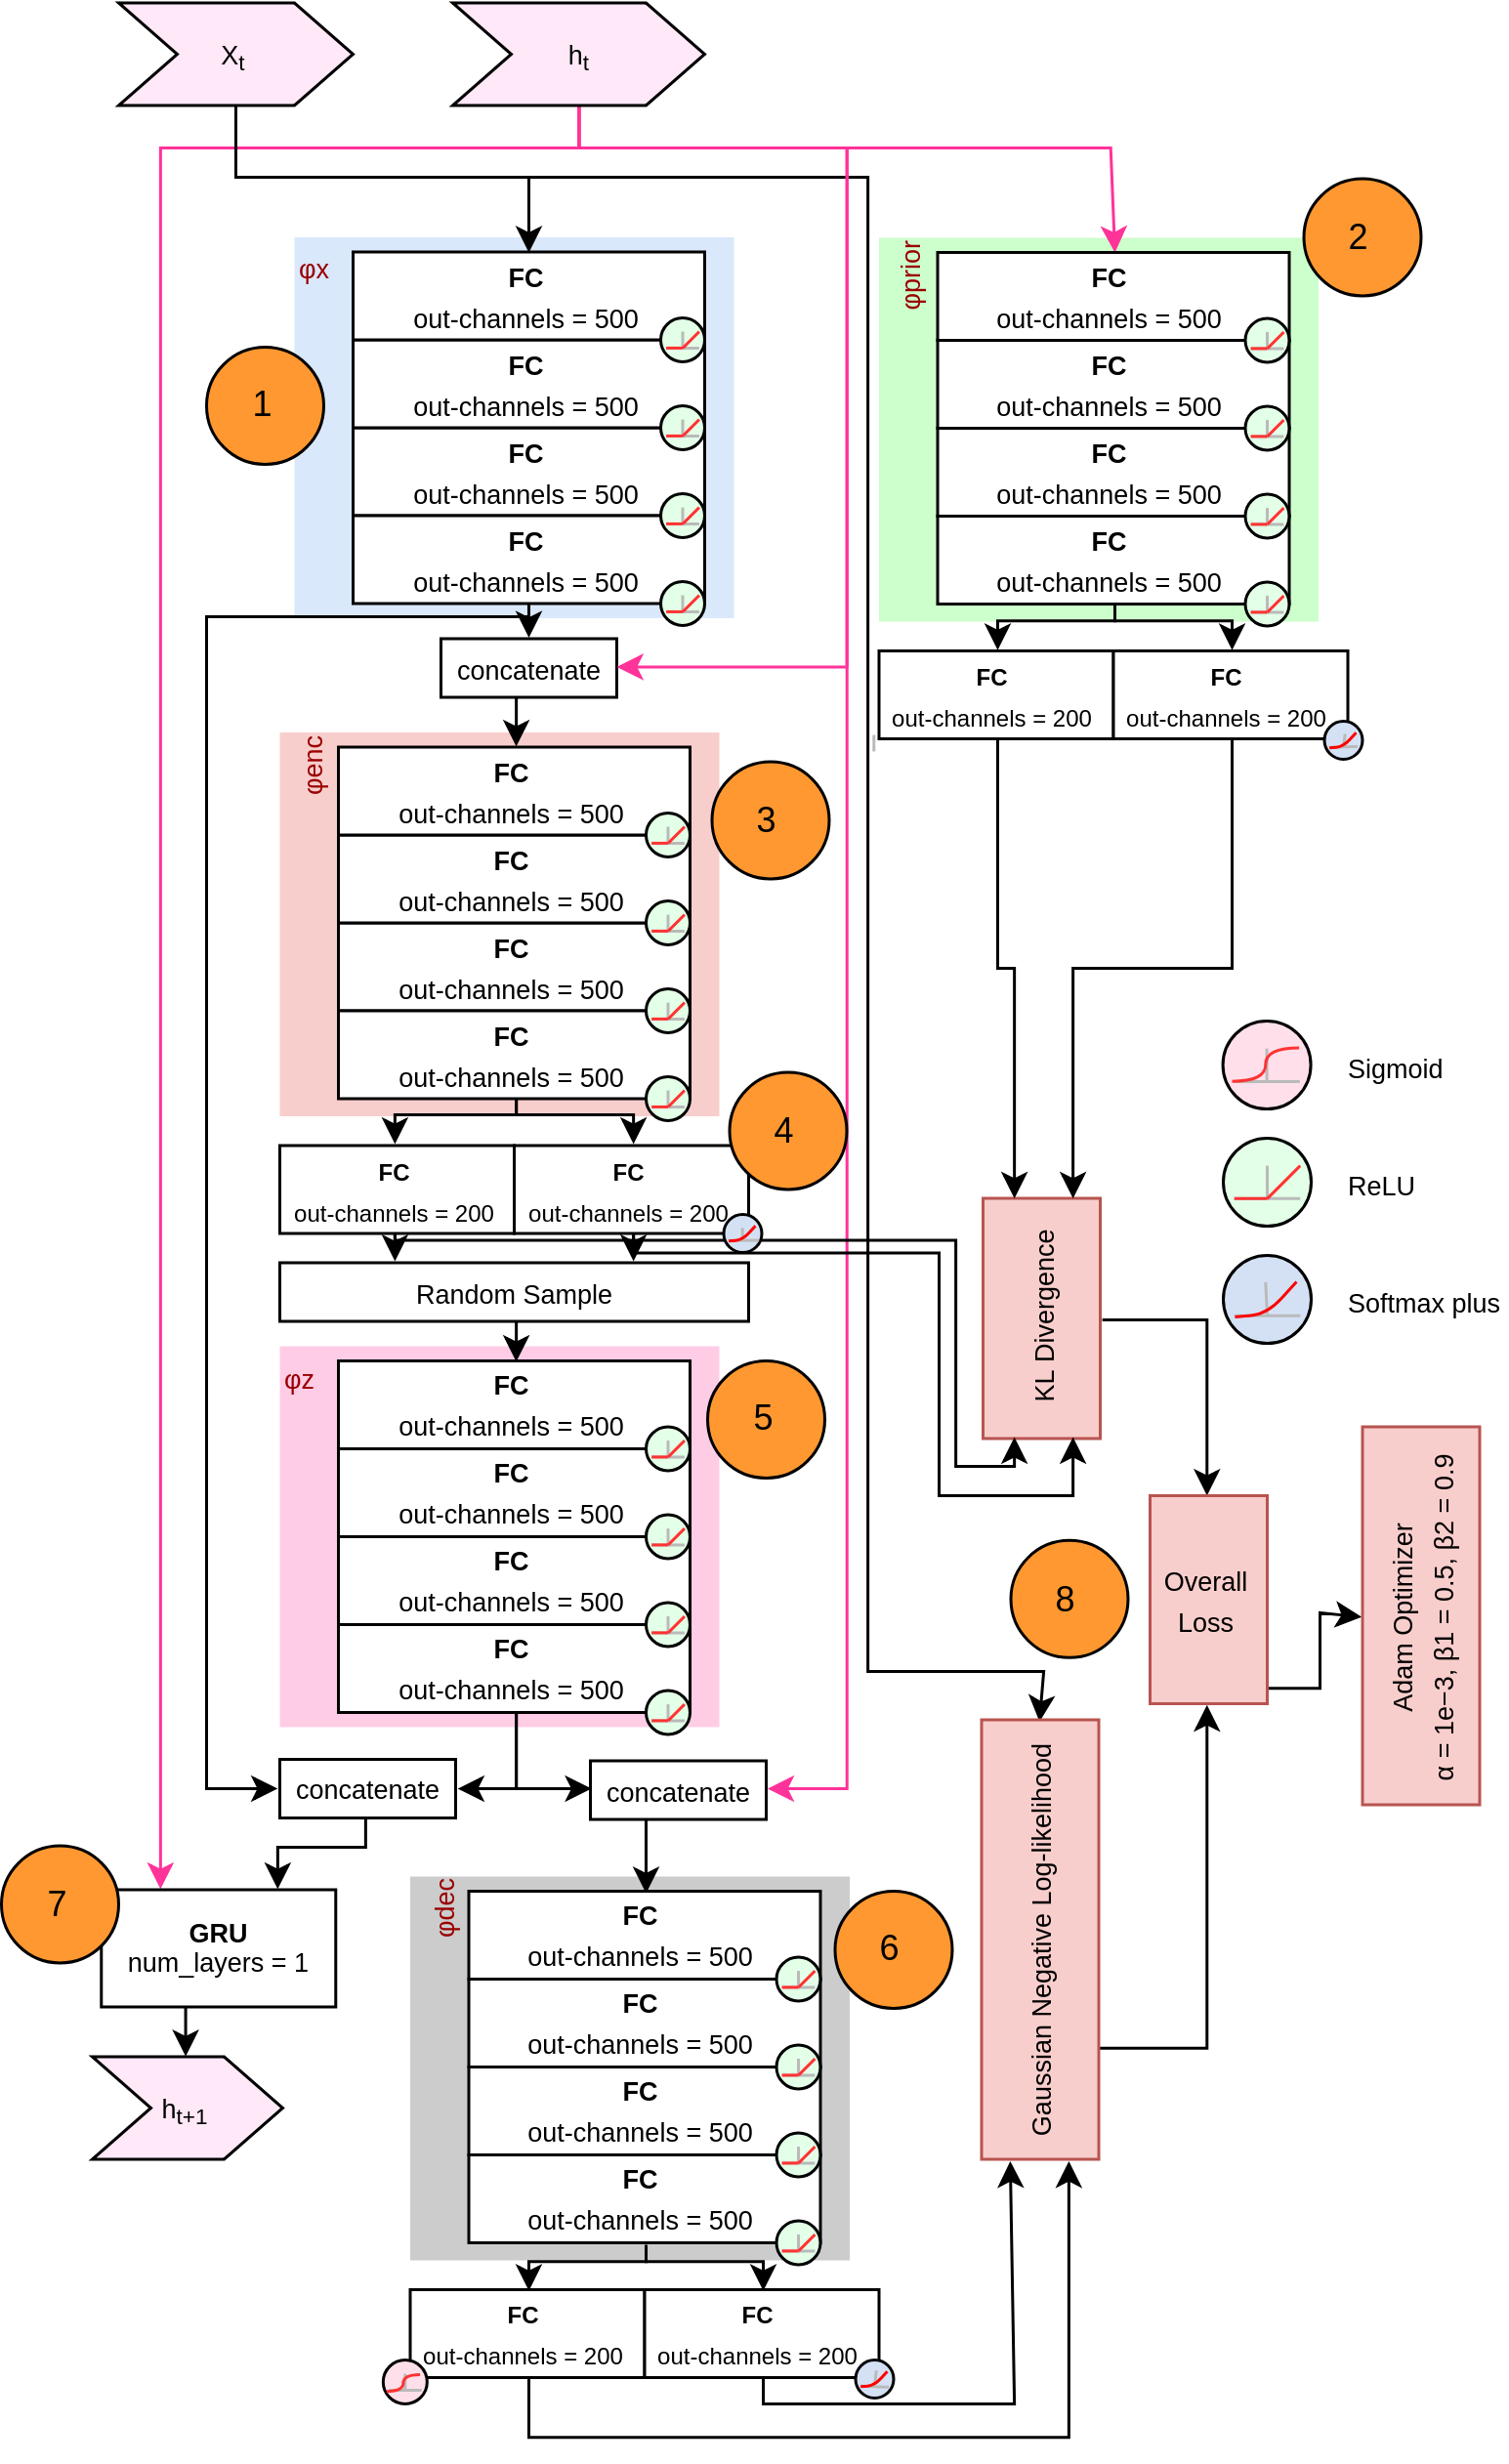
\includegraphics{vrnn-arch.png}
\label{fig:vrnn-arch}
\caption{
This image shows all necessary steps for a training cycle.
First the raw audio data is passed through $\phi^x$ to extract features from $x_t$ (1).
Since the KLD is used to make the $\phi^{prior}$ and $\phi^{enc}$ as similar as possible, the prior needs to be included in the model.
It handles the state vector $h_t$ (2).
The encoder $\phi^{enc}$ is used during training only.
It takes the concatenated $\phi^x$ and the state vector $h_t$ (3).
Next two single layer networks are used to calculate the standard deviation and the mean value of the generated distribution and a random sample $z$ is drawn from it (4).
Another network $\phi^z$ is used to find features in $z$ (5).
The decoder tries to replicate the mean and standard deviation of the input data. % ???
It takes the concatenated $\phi^z$ and $h_t$ (6).
$z$ and $h$ are passed to the RNN to determine a new state vector $h_{t+1}$ (7).
Lastly the overall loss is calculated (8).
It is composed of the KLD from $\phi^{prior}$ and $\phi^{dec}$ to make them similar, as well as a function to compare $x$ to $x:out$ % ???
}
\end{figure}





% Describe p, q, ...

conditional prior / generative model - p(x | z)
approximate posterior / inference model - q(z | x)
prior over latent random variables - p(z)


The model can be trained by minimizing the Kullback–Leibler divergence (KLD) - first term - and maximizing the likelihood of an $x$ given a $z$ - second term).
This can be seen as adding a regulizer to a simple auto encoder to ensure that the generated distributions have a certain form.
$$
E_{\mathbf{z} \le T | \mathbf{x} \le T} = \left[ \sum_{t=1}^T -(KL(q(\mathbf{z}_t | \mathbf{x}_{\le t}, \mathbf{z}_{<t}) || p(\mathbf{z}_t | \mathbf{x}_{<t}, \mathbf{z}_{<t})) + log(p(\mathbf{x}_t | \mathbf{z}_{\le t, \mathbf{x}_{<t}}))) \right]
$$

The KLD between the two distributions $Q$ and $P$ with respect to $Q$ can be seen as a measurment of similarity between two distributions \cite{}.
Since the probabilistic Encoder $q(z|x)$ is used to approximate the hard to compute posterior $p(x|z)$, $Q$ needs to be as similar to $P$ as possible.
This means that the KL divergence needs to be minimized, which is identical to maximizing the lower variational bound~\cite{kingma2013auto}. 
%The KLD is defined as:
%$$
%KL(q || p) = -\sum p(x) log(\frac{p(x)}{q(x)})  
%$$

The second term of the error function describes the reconstruction error.
%$$
%log p(\mathbf{x}_t | \mathbf{z}_{\le t, \mathbf{x}_{<t}})
%$$

In theory the model can be trained using any probability distribution.
The original paper uses gaussian distributions, leading to
$$
KL(q(\mathbf{z}_t | \mathbf{x}_{\le t}, \mathbf{z}_{<t}) || p(\mathbf{z}_t | \mathbf{x}_{<t}, \mathbf{z}_{<t}))
= \sum \frac{log(\sigma_2)}{log(\sigma_1)}+\frac{\sigma_1^2 + (\mu_1 - \mu_2)}{2 \sigma_2^2} - \frac{1}{2}
$$
for term 1, where $\mu_1$ and $\mu_2$ are mean values and $\sigma_1$ and $\sigma_2$ are are the standard deviations of the two distributions $p$ and $q$ (see \cite{klproof} for a proof ), and
$$
log(p(\mathbf{x}_t | \mathbf{z}_{\le t, \mathbf{x}_{<t}}))
= \sum \frac{\sqrt{y-\mu}}{2 \sigma^2} + log(\sigma) + \frac{log(2\pi)}{2}
$$
describes the second term, where %To_do!


% Implementierungsdetaills
Since the original source code was using the Theano ML library, I cloned a public PyTorch implementation~\cite{VRNNgit}.
However, I found out, that I needed to make quite many adaptions to fit the original version.
The biggest changes include a new data loader class, adding the correct error function, using more dense layers in all components and make the code more GPU-friendly. 


% Results

\subsubsection{Architecture}
\subsubsection{Training}









\section{WaveGAN}
In 2014 Goodfellow et al. introduced a new approach to train networks called Generative Adversarial Networks (GANs)~\cite{goodfellow2014generative}.
Such architectures consist of a generator and a discriminator sub-network.
While the discriminator tries to distinguish between real and generated data, it is the generator?s task to fool the discriminator into thinking its output is real.
Both networks are trained simultaneously and try to outperform each other.

While GANs have been used widely for tasks related to images, there are only few approaches using audio data.
Donahue et al. presented two GAN approaches to generate sound data called \emph{WaveGAN} and \emph{SpecGAN}~\cite{donahue2018adversarial}.
Both models are adaptions of a model class called Deep Convolutional Generative Adverserial Networks or DCGANs, first proposed by Radford et al.~\cite{radford2015unsupervised}.
The SpecGAN works with spectrogram images that are processed by the network in a similar way to normal images.
However, the final conversion from image to sound data is known to be problematic, since a lot of noise is induced.
The second architecture, the WaveGAN, is a flattened adaption of the original DCGAN model using 1D convolutions on raw audio samples.
Both models have the same number of parameters and numerical operations.
However, neither strategy has been tested with music datasets.
Since SpecGANs lossy conversion poses difficulties beyond the actual AI model, only the second approach will be presented here.

Unfortunately the original model description is only capable to generate about a second of audio.
By adding one more transposed convolution layer to the encoder, one convolution layer to the decoder, and increasing the number of intermediate output channels, the models generating capacity can be increased to about 4 seconds, possibly
enabling whole musical motifs. 
This expanded model can be found on the authors GIT repository\cite{donahue2019wavegan}.



\subsection{Architecture}
The generator network is trained to map a low-dimensional latent vector $z$ to a high-dimensional data output.
First the network applies a fully connected layer with $512d$ output nodes to $z$, where $d$ is used to adjust the models size.
The output vector is then reshaped, since an additional dimension is needed for the sound channel.
The signal then passes through 5 transposed 1D convolution layers with stride 4 and ReLU activation functions in between as well as a Tanh function at the end.

The decoder is basically a mirrored generator with a few exceptions.
Instead of ReLUs, Leaky ReLUs with $\alpha=0.2$ are used in between convolution layers.
Also a new kind of layer, called PhaseShuffle, is introduced here. 
Since the generators transposed convolution is known to produce artifacts, the discriminator may learn to find generated samples based on these artifacts instead of conducting a broad content analysis.
Shifting the vector randomly up to $n$ times in a circle can prevent this learning behaviour.
See figure \ref{fig:WaveGan-arch} for a visualization of the graph with parameters.


% To-Do!
\begin{figure}[ht!]
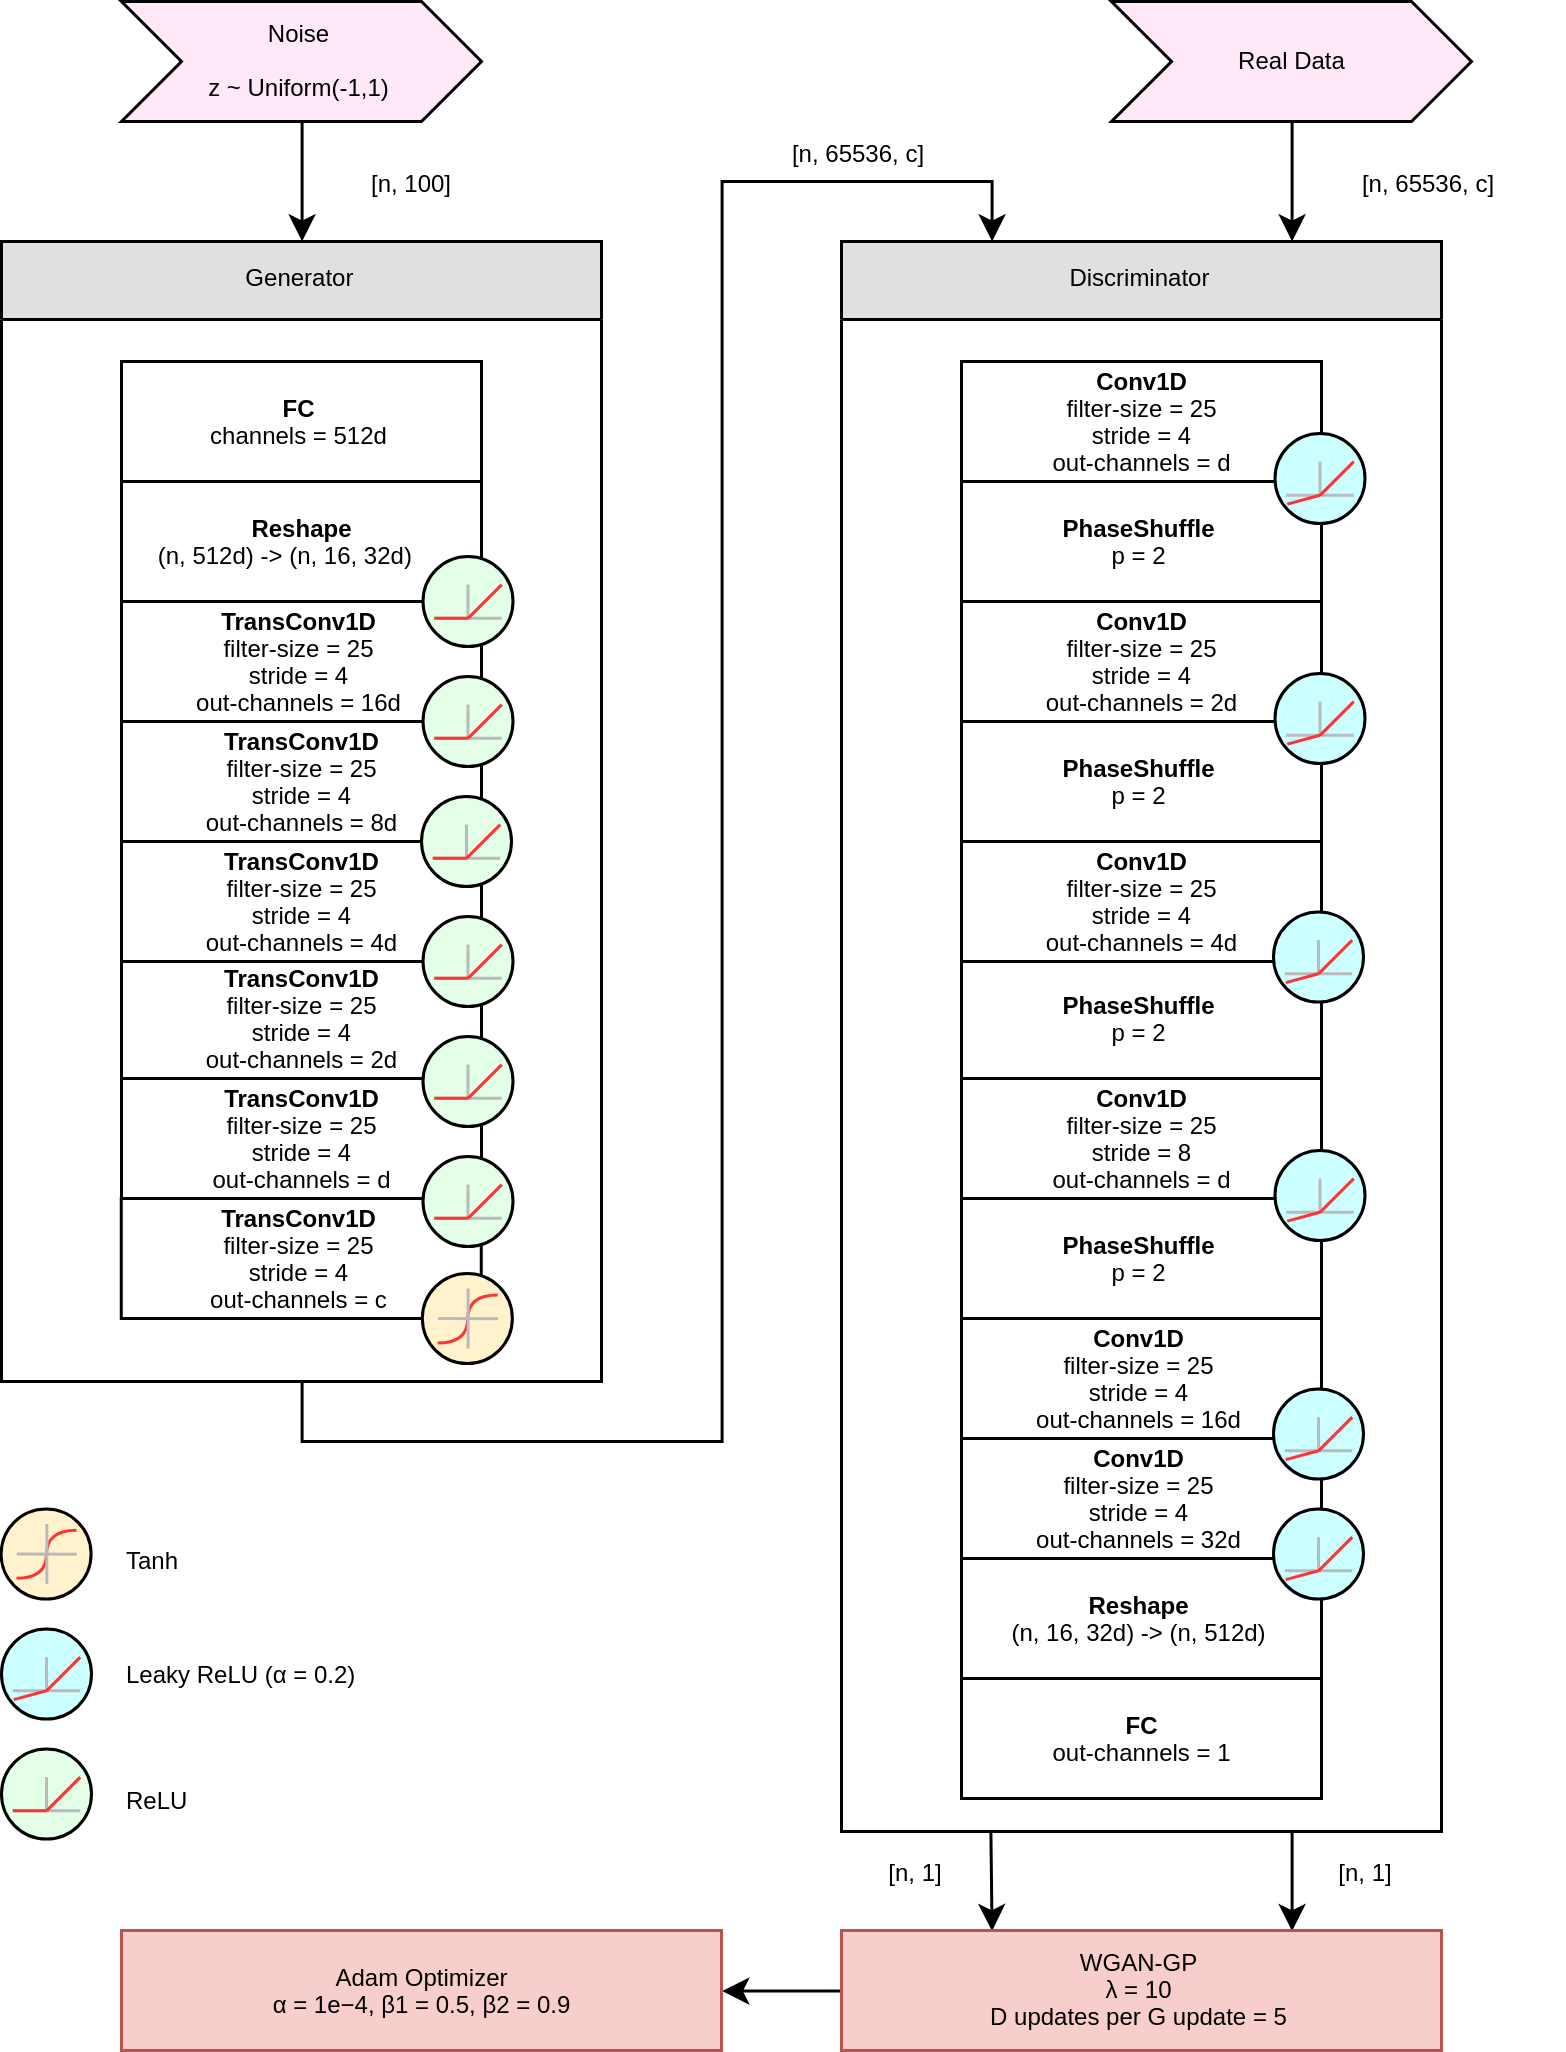
\includegraphics[width=0.9\textwidth]{img/wavegan-arch.png}
\caption{Architecture of the WaveGAN, where $d$ adjusts the models size, $n$ is the batch size and $c$ is the number of output channels.}%To-Do
\label{fig:WaveGan-arch}
\end{figure}

\subsection{Training}

Training GANs can be seen as a two player minimax game. 
While the generator $G$ is trained to minimize the following value function, the discriminator
$D_w$ is trained to maximize it.

$$
V_{WGAN}(D_w, G) = E_{x \sim P_x}[D_w(x)] - E_{z \sim P_z}[D_w(G(z))]
$$

The network is trained using the Wasserstein-GAN Gradient Penalty, or short \emph{WGAN-GP}, strategy.
That means, that instead of predicting probabilities, the discriminator is trained to assist computing the wasserstein or
earth movers distance between the distribution of generated data and distribution of real examples.
However, minimizing this measure is only possible if the discriminator function is 1-Lipschitz, which can be done by enforcing a gradient penalty.
For more details on the WGAN-GP stategy see~\cite{gulrajani2017improved}.

In most experiments training was stopped in between $40.000$ and $50.000$ steps since no more progress was achieved.
On a NVIDIA RTX2080 GPU, this took about a day and 7 of 8Gb RAM.
All other parameter choices are similar to \cite{donahue2018adversarial}.
Adam Optimizer with $learning rate = 1e ? 4$, $?1 = 0.5$ and $?2 = 0.9$
was used for both discriminator and generator.
The model was trained using both a batch size $b$ and a scale factor $d$ of 64.


\section{Evaluation}
SampleRNN, VRNN and WaveGAN have been rained on
\begin{itemize}
 \item piano music (Felix Mendelssohn: Lieder ohne Worte, about 2 hours)
 \item instrumental metal (Intervals: The Way Forward + A Voice Within + In Time, 1 hour and 53 minutes) % To-DO
 \item hip-hop (Cypress Hill: Cypress Hill, 46 minutes)
\end{itemize}

For SampleRNN and VRNN the music was split into 8 second and for WaveGAN into 4 second chunks.
Audio examples can be found in the repository folder examples. % TO-DO!



% SampleRNN
In our experiments SampleRNN always produced the cleanest sound.
Despite its relative complicated architecture, the model learned to produce first musical features like drum hits and screams after only about 5 minutes of training.
However, it takes much more training to reduce noise and generate more complex features like guitar riffs.
The models biggest drawback is, that sample quality varies strongly even after days of training.
In a few experiments the model even completely regressed to produce sound or white noise only.
This was also described by \cite{carr2018generating} who advised to restart training if output samples during training remain bad.
Future work should investigate how to avoid this unpredictable behaviour.
Another drawback of the SampleRNN is the long music generation time since every genration cicle outputs a single sample that needs to be fed back into the model.
With the architecture described above it takes about <20> minutes to generate 2 minutes of audio. % To-do!
However, assuming that there is enough memory, increasing generation batch size does not affect the overall generation time since it can be parallelized.

% -  causing the loss values to shoot up and the resulting audio to revert to static. (sogar im Orginal!)

% WaveGAN
Despite GANS being often hard to train, WaveGAN has the most simple architecture out of all three models.
Unlike both other autoregressive models, where samples have to be fed back into the model, the WaveGAN audio generation is feed-forward only, which makes generation extremely fast.
It also is the only architecture that is (out-of-the-box) capable of producing multi-channel sound output.
However, the main drawback of the WaveGAN is the models limitation to generate music of more than a couple seconds.
Regarding memory and complexity requirements compared to the other models, WaveGAN is very hard to scale.
In all experiments the model did learn to produce music that somewhat showed features from the input data.
In Samples one can often observe instruments, small riffs and drum hits.
However, in all experiments the networks never fully learned to reduce noise.
This can clearly be heard in the examples and often even dominates them.
Increasing the model and batch size on a GPU with more RAM might help.

\newpage
\bibliographystyle{plain} % Literaturverzeichnis
\begin{btSect}{doc} % mit bibtopic Quellen trennen
\section*{Sources}
\btPrintCited
\end{btSect}


\end{document}
